% === VII. Implementasi Perangkat Lunak ===
\secbox{VII.}{Implementasi Perangkat Lunak}

\subsecbar{7.1 Implementasi Teknologi}
Implementasi LUNA memanfaatkan kombinasi teknologi modern untuk mendukung komunikasi \textit{real-time}, pemrosesan kecerdasan buatan, penyimpanan data, serta pengalaman pengguna yang responsif. Rincian teknologi yang digunakan ditunjukkan pada Tabel 2.

\begin{table}[H]
\centering
\renewcommand{\arraystretch}{1.35}
\renewcommand{\tabularxcolumn}[1]{m{#1}}
\arrayrulecolor{TableBorderColor}
\caption{Implementasi Teknologi LUNA}
\vspace{0.3em}
\small
\begin{tabularx}{\textwidth}{| >{\bfseries\itshape}l | X |}
\hline
\rowcolor{TableHeaderPurple}
\color{white}\bfseries Komponen & \color{white}\bfseries Fungsi \\
\hline
Mobile Application (Flutter) & Pengembangan aplikasi Android dan iOS \\
\hline
\rowcolor{TableAltRowBg}
Backend Service (FastAPI) & REST API, WebSocket, dan orkestrasi Multi-Agent AI \\
\hline
Artificial Intelligence (DeepSeek LLM) & Menghasilkan respons percakapan yang natural dan kontekstual \\
\hline
\rowcolor{TableAltRowBg}
Speech-to-Text (OpenAI STT) & Mengubah suara menjadi teks \\
\hline
Text-to-Speech (OpenAI TTS) & Menghasilkan respons suara yang natural \\
\hline
\rowcolor{TableAltRowBg}
AI Architecture (Multi-Agent AI) & Mengelola kolaborasi antar agen AI \\
\hline
Knowledge Retrieval (RAG) & Mengambil referensi kesehatan mental yang relevan \\
\hline
\rowcolor{TableAltRowBg}
Vector Database (Qdrant) & Penyimpanan embedding dan pencarian semantik \\
\hline
Database (PostgreSQL) & Penyimpanan data pengguna, diary, dan riwayat percakapan \\
\hline
\rowcolor{TableAltRowBg}
Cache (Redis) & Penyimpanan sesi dan cache percakapan \\
\hline
Long-term Memory (Memory Worker) & Menyimpan preferensi dan konteks pengguna \\
\hline
\end{tabularx}
\end{table}

\subsecbar{7.2 Alur Penggunaan Sistem}
Alur penggunaan LUNA menjelaskan proses interaksi end-to-end antara pengguna dan sistem dalam memanfaatkan seluruh fitur utama. Secara rinci, alur operasional terdiri dari empat tahapan utama:
\begin{enumerate}[leftmargin=*,label=\arabic*.]
    \item \textbf{Autentikasi \& Onboarding}: Pengguna melakukan registrasi/login dan menyetujui etika layanan serta \textit{medical disclaimer}.
    \item \textbf{Dashboard \& Mood Monitoring}: Pengguna mencatat emosi harian (\textit{mood tracker}) dan memantau perkembangan tren kondisi emosional.
    \item \textbf{Konseling Interaktif (Teks \& Suara)}: Pengguna berinteraksi dalam sesi percakapan real-time dengan agen AI berbasis CBT.
    \item \textbf{Sintesis Jurnal \& Safety Gates}: Sistem backend secara otomatis merangkum jurnal harian, memantau tingkat risiko emosional, serta memicu intervensi darurat jika terdeteksi situasi krisis (\textit{High Risk}).
\end{enumerate}

Rangkaian alur penggunaan sistem tersebut disajikan pada Gambar 5.

\begin{figure}[H]
    \centering
    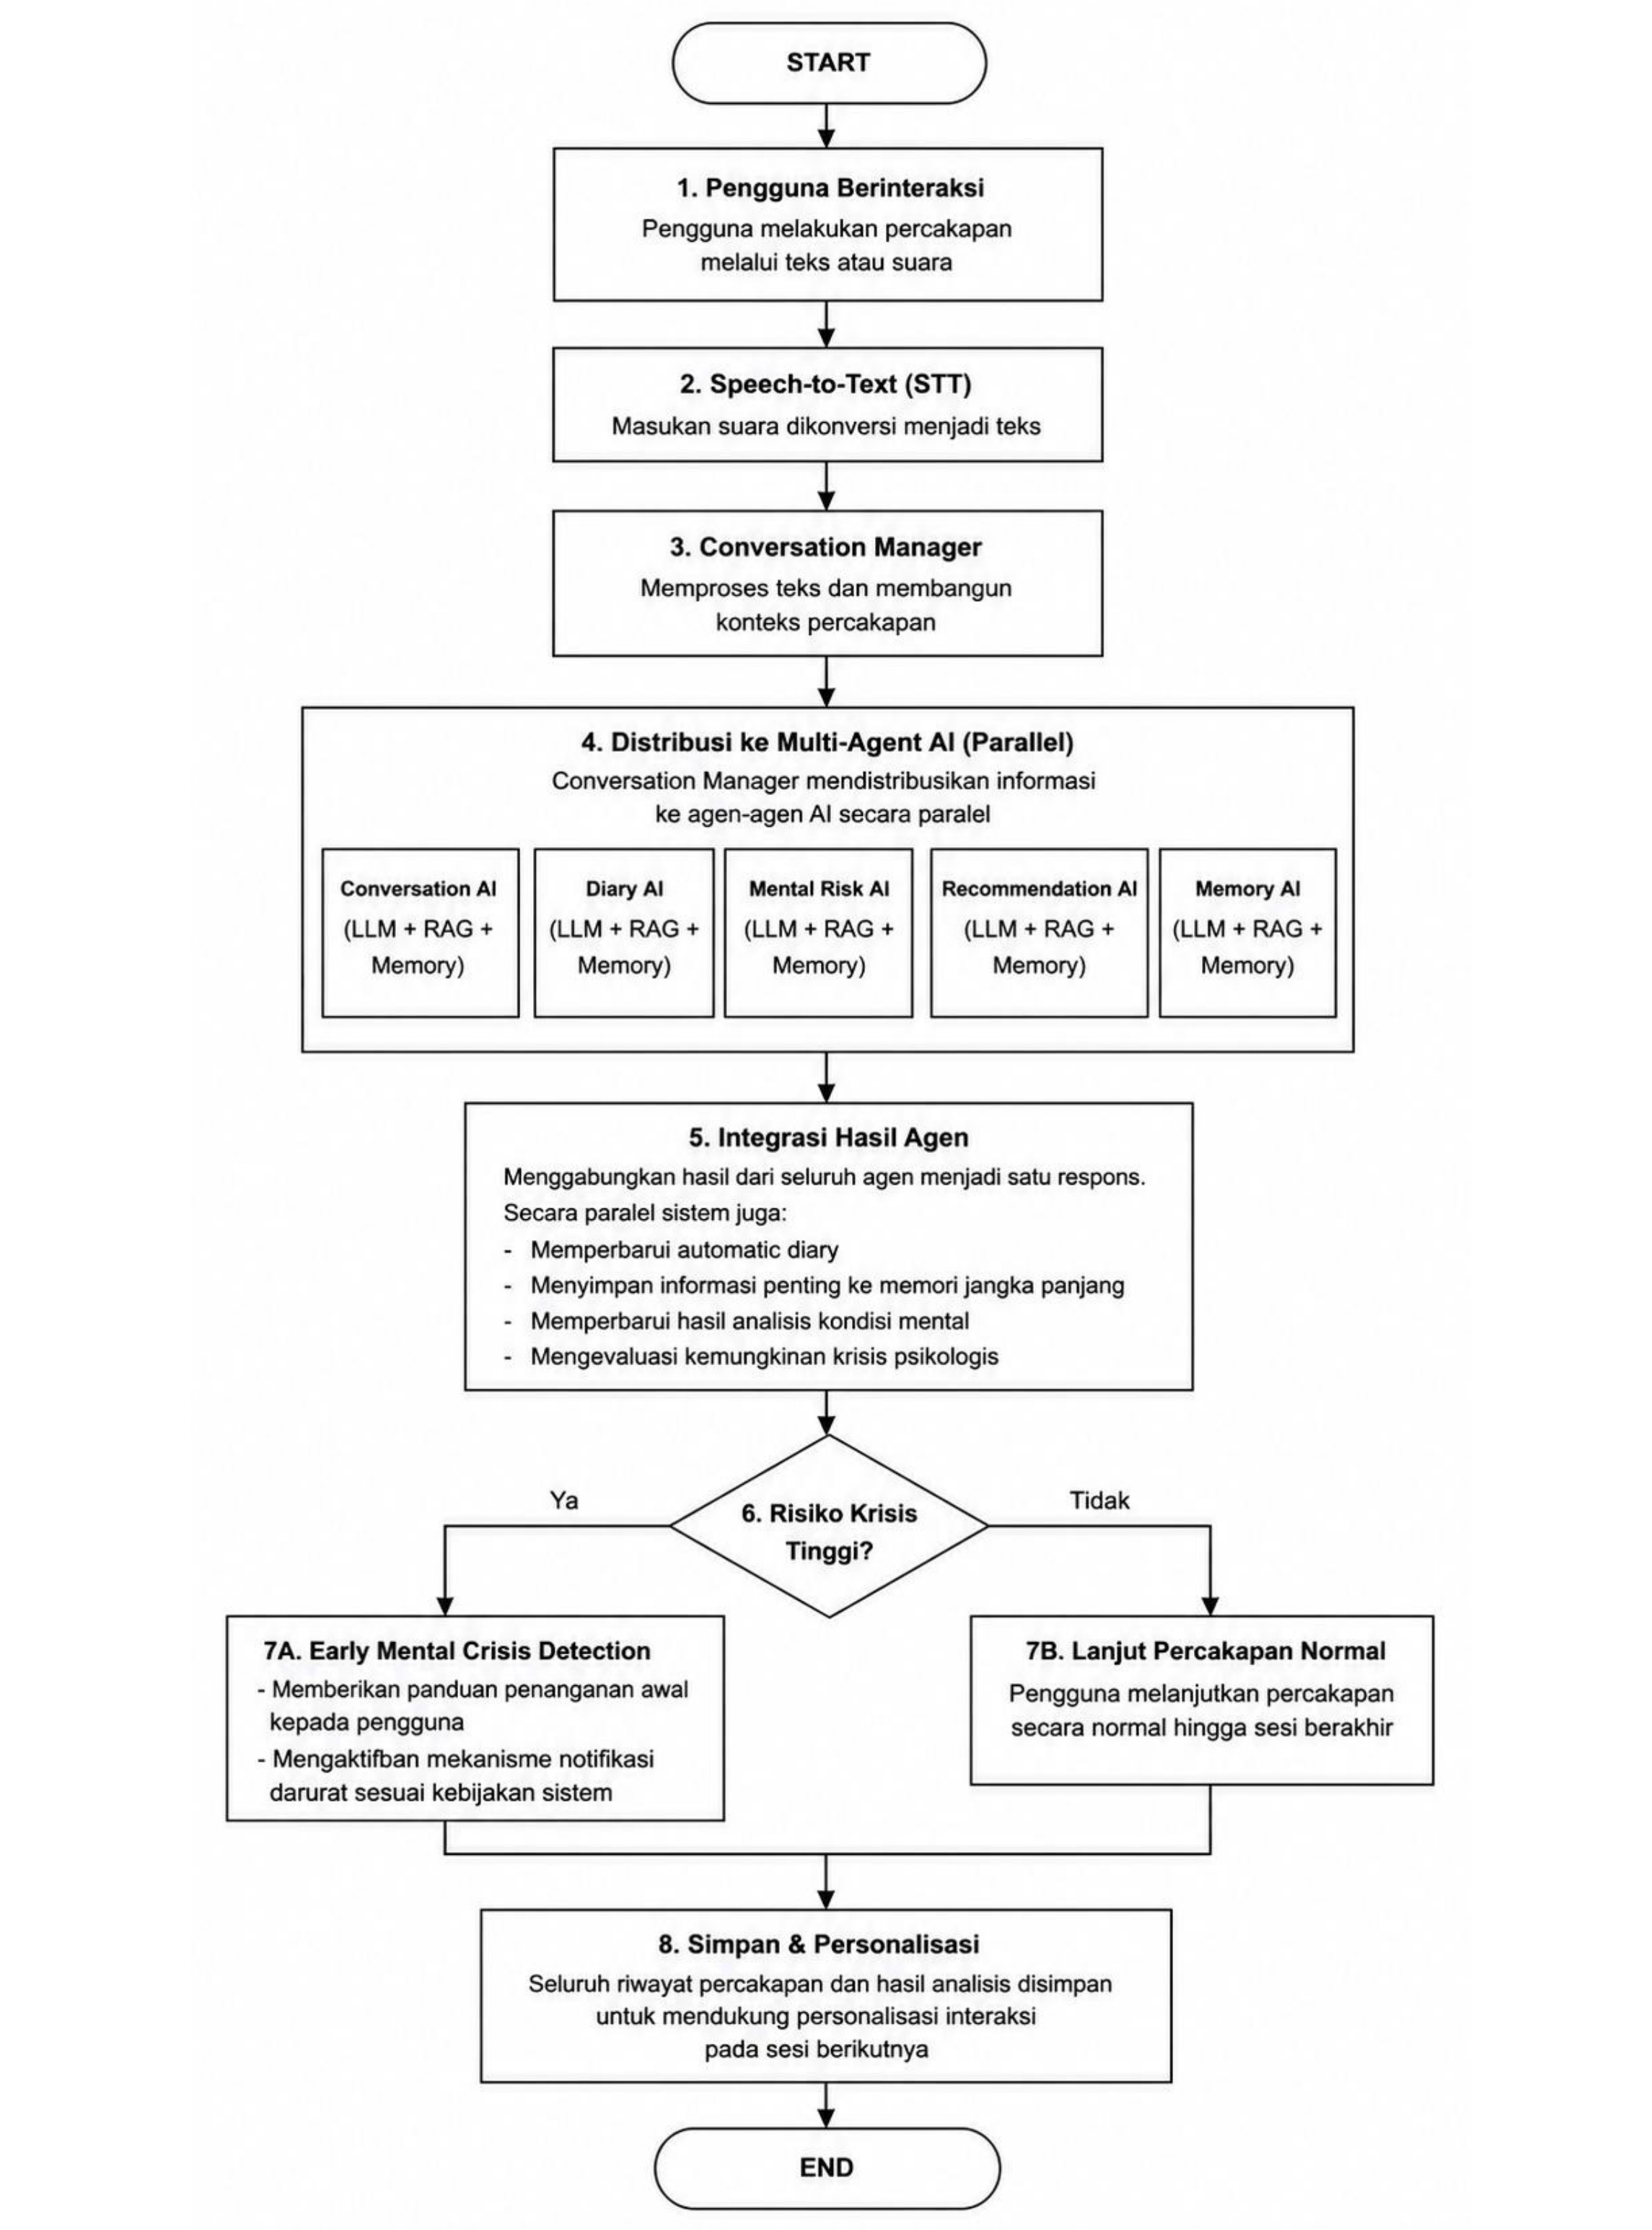
\includegraphics[height=17.5cm,keepaspectratio]{images/bab7/fig5_flow.png}
    \caption{Alur Penggunaan Sistem}
\end{figure}

\subsecbar{7.3 Peran Sistem}
Peran setiap aktor dalam LUNA dirancang untuk mendukung proses pendampingan kesehatan mental secara terintegrasi. Pembagian peran antara pengguna, sistem, komponen Multi-Agent AI, dan layanan notifikasi ditunjukkan pada Tabel 3.

\begin{table}[H]
\centering
\renewcommand{\arraystretch}{1.35}
\renewcommand{\tabularxcolumn}[1]{m{#1}}
\arrayrulecolor{TableBorderColor}
\caption{Peran Sistem}
\vspace{0.3em}
\small
\begin{tabularx}{\textwidth}{| >{\bfseries}l | X |}
\hline
\rowcolor{TableHeaderPurple}
\color{white}\bfseries Aktor & \color{white}\bfseries Peran \\
\hline
Pengguna & Melakukan percakapan melalui teks maupun suara, melihat diary, melihat riwayat, menerima rekomendasi, dan memantau kondisi mental. \\
\hline
\rowcolor{TableAltRowBg}
LUNA & Memberikan pendampingan psikologis awal melalui percakapan yang personal dan adaptif. \\
\hline
Multi-Agent AI & Mengelola percakapan, menyusun diary, menganalisis risiko mental, memberikan rekomendasi, serta mengelola memori percakapan. \\
\hline
\rowcolor{TableAltRowBg}
Notification Center & Mengirimkan notifikasi ketika terdeteksi potensi krisis mental sesuai kebijakan sistem. \\
\hline
\end{tabularx}
\end{table}
